\newpage
\section{TGGs in action}
\genHeader
\label{sect:TGGs_in_Action}
In this section, we shall export our TGG, implement our new constraint, and get our integration running!

\begin{enumerate}
\item[$\blacktriangleright$] Export your metamodels and TGG by choosing ``\texttt{Extensions/\-MOFLON::\-Ecore Addin\-/Export all to Workspace}'' as usual in EA and refres your Eclipse Metamodel project to trigger code generation.
\end{enumerate}

If you have done everything right, code generation and compilation should terminate without any error and the structure of the \texttt{gen} folder in \texttt{LearningBox\-To\-Dictionary\-Integration} should resemble Fig.~\ref{fig:gen_folder}.

\begin{figure}[htbp]
\begin{center}
  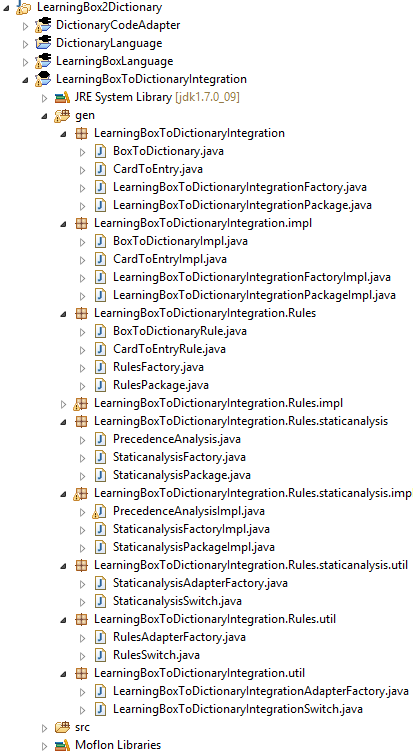
\includegraphics[width=0.6\textwidth]{tgg22}
  \caption{Integration project after code generation}
  \label{fig:gen_folder}
\end{center}
\end{figure}

\begin{enumerate}
  \item[$\blacktriangleright$] To implement our constraint \texttt{IndexToLevel}, locate and open the file \texttt{csp/IndexToLevel.java} in the \texttt{src} folder of \texttt{Learning\-Box\-To\-Dictionary\-Integration}.
  \item[$\blacktriangleright$] Insert the code provided in Fig.~\ref{fig:indexToLevel}

\end{enumerate}

\begin{figure}[htbp]
\begin{center}
  % 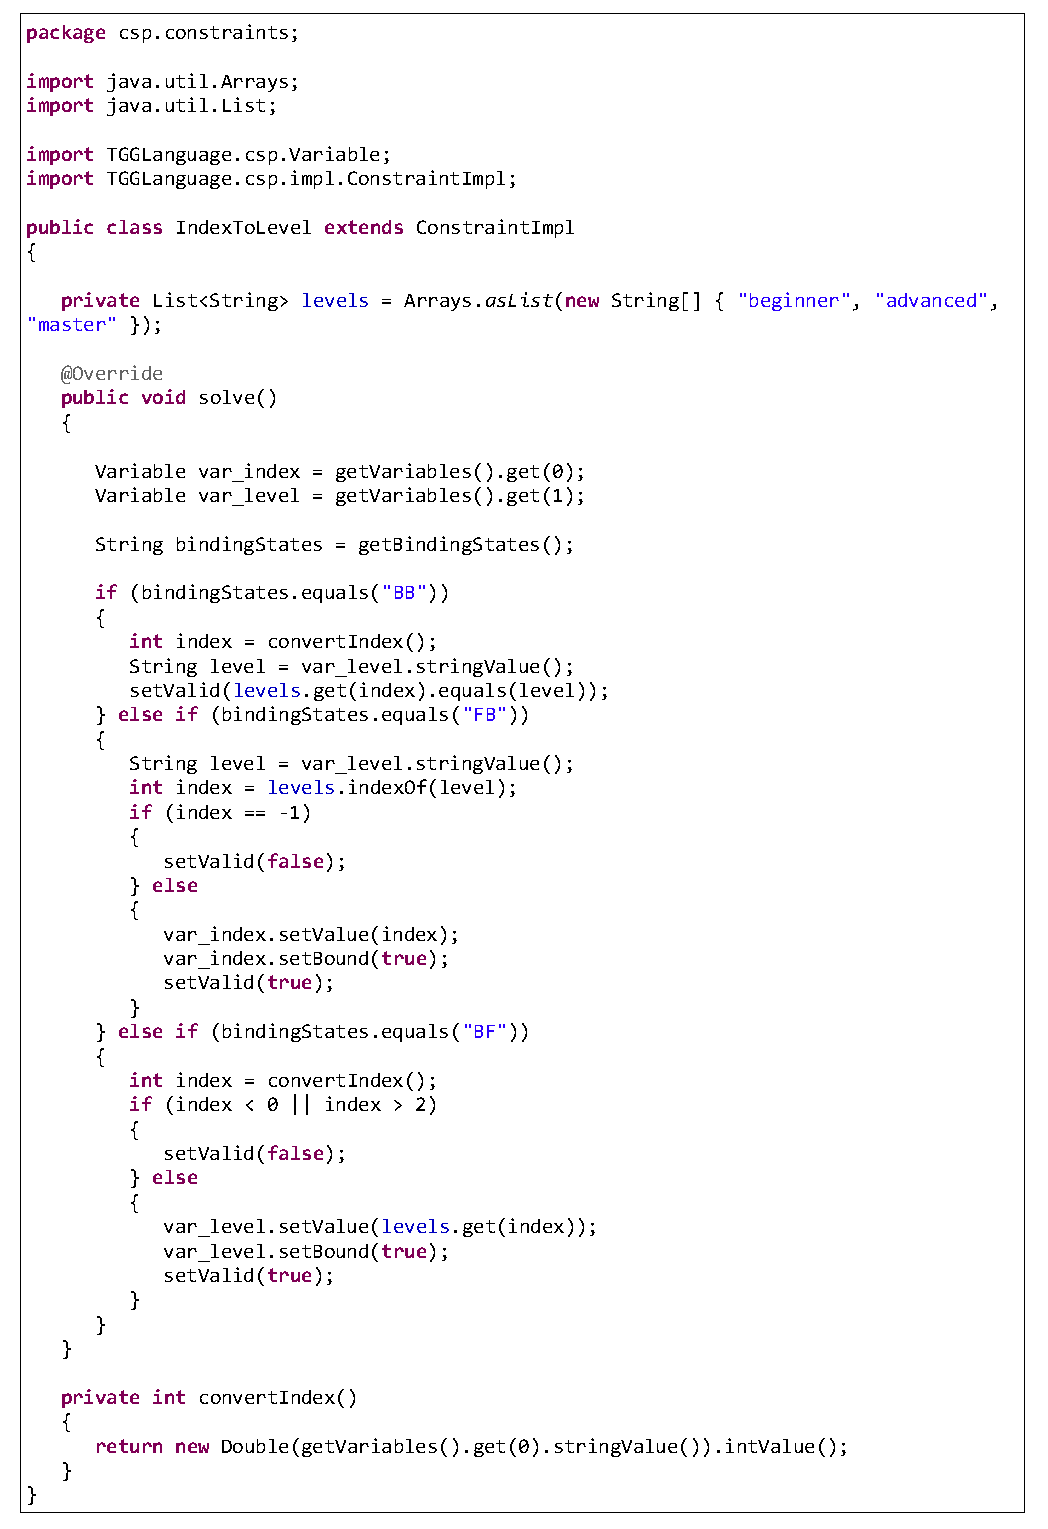
\includegraphics[height=0.64\textheight]{pics/tggBilder/transformation/tgg23}
\begin{lstlisting}[language=Java,backgroundcolor=\color{white}, keywordstyle={\bfseries\color{purple}}]
package csp.constraints;

import java.util.Arrays;
import java.util.List;

import TGGLanguage.csp.Variable;
import TGGLanguage.csp.impl.ConstraintImpl;

public class IndexToLevel extends ConstraintImpl {

  private List<String> levels = Arrays.asList(new String[] { "beginner",
      "advanced", "master" });


  public void solve(Variable<Integer> var_0, Variable<String> var_1){
    String bindingStates = getBindingStates(var_0, var_1);

    switch(bindingStates){
    case "BB":
      int indexBB = var_0.getValue().intValue();
      String level = var_1.getValue();
      setSatisfied(levels.get(indexBB).equals(level));
      break;
    case "BF":
     int indexFB = var_0.getValue().intValue();
      if (indexFB < 0 || indexFB > 2) {
        setSatisfied(false);
      } else {
        var_1.setValue(levels.get(indexFB));
        var_1.setBound(true);
        setSatisfied(true);
      }
      break;
    case "FB":
      String levelBF = var_1.getValue();
      int indexBF = levels.indexOf(levelBF);
      if (indexBF == -1) {
        setSatisfied(false);
      } else {
        var_0.setValue(indexBF);
        var_0.setBound(true);
        setSatisfied(true);
      }
      break;
    }

  }
}
\end{lstlisting}
  \caption{Implementation of our attribute constraint}
  \label{fig:indexToLevel}
\end{center}
\end{figure}

In the next few steps, we shall create an instance model\footnote{Refer to Chapter \ref{sect:instance} if you do not know how to do this.} of one of our languages and  transform it to an instance model of the other language according to our TGG, i.e., perform a forward and backward transformation.
As dictionaries are of a much simple structure, let's start with a backward transformation, i.e., dictionary to learning box:

\begin{enumerate}
\item[$\blacktriangleright$] Open \texttt{Dictionary\-Language/model/Dictionary\-Language.ecore} and create a dynamic instance of \texttt{Dictionary}, and save it under \texttt{Learn\-ing\-Box\-To\-Dictionary\-In\-te\-gra\-tion/in\-stan\-ces/target.xmi} (Fig.~\ref{fig:create_instance_dict}).

\begin{figure}[htbp]
\begin{center}
  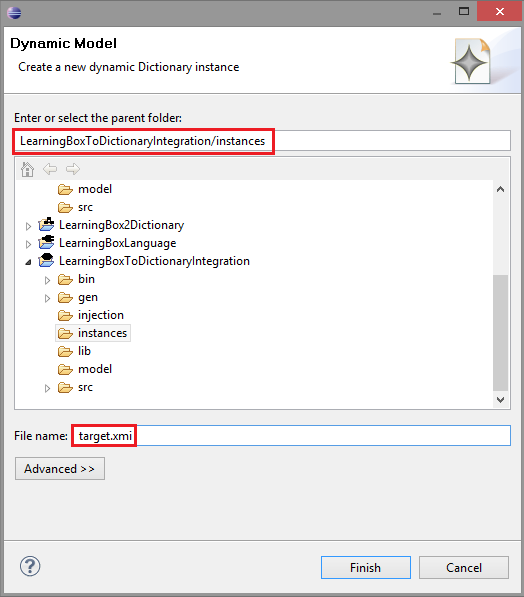
\includegraphics[width=0.7\textwidth]{tgg24}
  \caption{Create a dynamic instance of \texttt{Dictionary}}
  \label{fig:create_instance_dict}
\end{center}
\end{figure}

\item[$\blacktriangleright$] Open \texttt{target.xmi} and set \texttt{Dictionary.title} to \texttt{English Numbers}.
\item[$\blacktriangleright$] Create two \texttt{Entry} objects as children of \texttt{Dictionary}: the first entry with \texttt{one : eins} as content and \texttt{beginner} as level, the second with \texttt{eleven : elf} as content and \texttt{advanced} as level (Fig.~\ref{fig:dictionaryxmi}).

\begin{figure}[htbp]
\begin{center}
  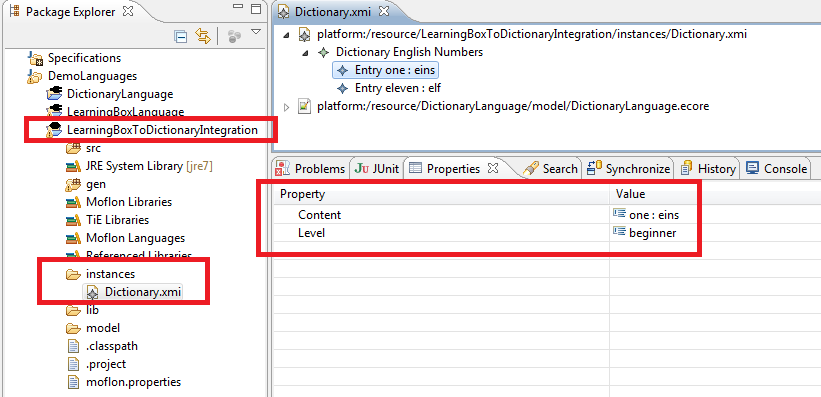
\includegraphics[width=\textwidth]{tgg26}
  \caption{Contents of the dictionary}
  \label{fig:dictionaryxmi}
\end{center}
\end{figure}

\item[$\blacktriangleright$] Run the automatically created main class \texttt{TGGMain} in \texttt{LearningBox\-To\-Dictionary\-In\-te\-gra\-tion\-/src} and refresh the folder \texttt{LearningBox\-To\-Dictionary\-In\-te\-gra\-tion/\-instances}. 

Note the error message ``Unable to load instances/source.xmi, instances/source.xmi does not exist.'' in the console.
This is because no source file was found for the forward transformation.
We'll fix that in a moment.
\end{enumerate}

As you can see, our \texttt{Dictionary} has been backward translated to a \texttt{Box} with the same name (\texttt{English Numbers}), containing three \texttt{Par\-ti\-tions}, as specified in \texttt{Box\-To\-Dictionary\-Rule}.
The two \texttt{Entry} objects have also been translated to \texttt{Card} objects as specified in \texttt{CartToEntryRule}.
Also note that the \texttt{face} and the \texttt{back} of the \texttt{Card}s are consistent with the \texttt{content} of the corresponding \texttt{Entry}, e.g. \texttt{card.face = ``Question : one''} and \texttt{card.back = ``Answer : eins''}.
The indices of the partitions containing the cards are also consistent with the level of the entry, i.e., \texttt{0} for \texttt{beginner}, and \texttt{1} for \texttt{advanced} 
(do not let the names of the partitions in the view confuse you: they are labelled using their size (all 0), and not their index, double-click the partitions to see the values of \emph{all} their attributes in the property window).

Congratulations! You have successfully performed your first \emph{backward} transformation from \texttt{Dictionary\-Language} (target model) to \texttt{Learn\-ing\-Box\-Lan\-guage} (source model) using TGGs!

To show that the transformation is actually bidirectional, lets edit the created source model and transform it \emph{forward} to a new target model:

\begin{enumerate}
\item[$\blacktriangleright$] Make a copy of \texttt{target.xmi\_BWD.xmi} (the result of the backward transformation)
and rename it to \texttt{source.xmi}.
  
\item[$\blacktriangleright$] Open \texttt{source.xmi} and create some new \texttt{Card} objects in the \texttt{Partition}s (e.g., create a new \texttt{Card} with \texttt{Card.face = ``Question : two''}, \texttt{Card.back = ``Answer : zwei''} in \texttt{Partition 0}).

\item[$\blacktriangleright$] Run the \texttt{TGGMain.java} again and inspect the 
created target model \texttt{source.xmi\_FWD.xmi} (result of the forward transformation). 

\end{enumerate}

To end this chapter on TGGs, lets take a look at a \emph{visualization} of the created triple of models:

\begin{enumerate}


\item[$\blacktriangleright$] Right-click on \texttt{corr\_BWD.xmi} and choose ``eMoflon $\rightarrow$ Start Integrator'', which opens the window depicted in Fig.~\ref{fig:integrator_start}.

\begin{figure}[htbp]
\begin{center}
  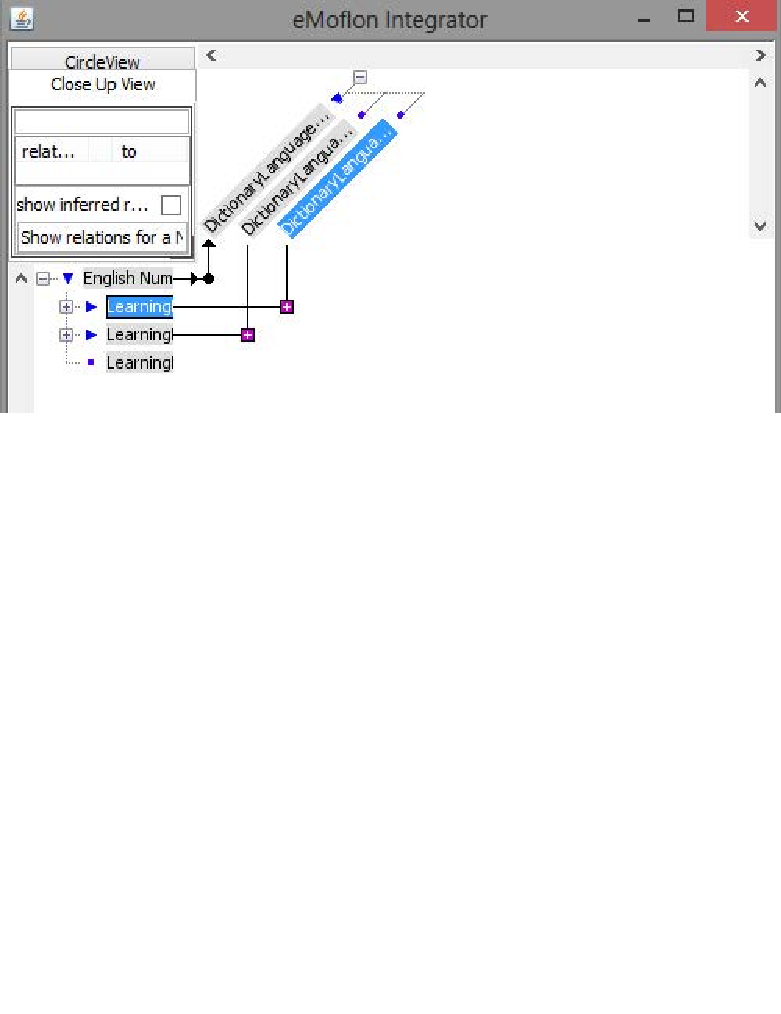
\includegraphics[width=0.7\textwidth]{integrator_start_view.pdf}
  \caption{Default view of the integrator}
  \label{fig:integrator_start}
\end{center}
\end{figure}

\item[$\blacktriangleright$] Drag and drop \texttt{protocol\_BWD.xmi} into the integrator window. 
You will now see the controls explained in the lower part of the window 
(Fig.~\ref{fig:integrator_after_protocol}). 
Note that this chapter will only cover the very basic commands so please refer to 
Appendix \ref{sec:app_integrator} for further information (e.g. about setting breakpoints).

\begin{figure}[htbp]
\begin{center}
  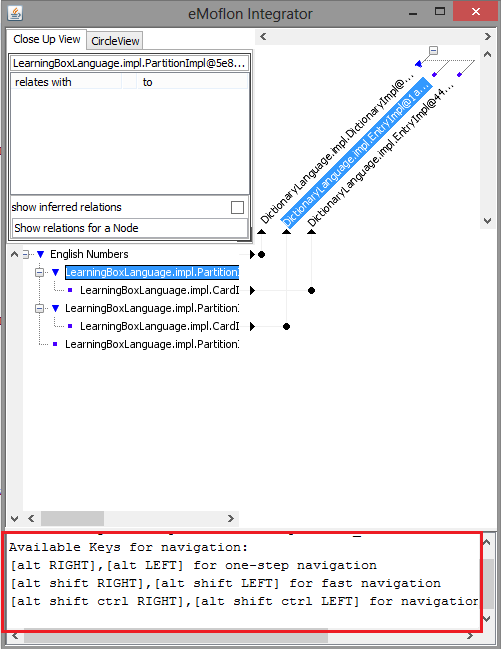
\includegraphics[width=0.7\textwidth]{integrator_after_protocol_insertion.png}
  \caption{Integrator after protocol insertion.}
  \label{fig:integrator_after_protocol}
\end{center}
\end{figure} 
\FloatBarrier

\item[$\blacktriangleright$] The integrator works as an ``offline'' debugger which works on the protocol 
(trace) of the transformation. 
You can use \texttt{Alt+Right} to navigate forwards through the transformation process and \texttt{Alt+Left} 
to go backwards. 
When you step through the transformation, you will notice that some elements are highlighted with colours. 
These are the elements that are currently being processed and the colours have the following meaning:
\begin{description}
  \item[Blue] The element is now about to be processed (is being ``looked at'').
  \item[Yellow] The element cannot be transformed right now and has been queued for later transformation 
  (e.g., when transforming an Entry to a Card, the Box with partitions to put the 
  Card into must be translated first).
  \item[Green] The object has just been created.
\end{description}
\end{enumerate}